\chapter{Work Completed}\label{C:work}

This chapter will discuss the work that has been completed so far on this project. It will begin by discussing the projects requirements', using them to design and justify the final specifications of the system. Once the specifications are outlined, the architecture and design of the final system will be discussed. Finally the design and current implementation of the PWM signal generator will be specified.  

\section{Defining \& Justifying System Specifications}\label{S:specs}

\begin{itemize}

    \item 
    Discuss the requirements that were laid out in the project proposal for the evaluation of the system. 

    \item 
    Discuss how these system requirements needed to be translated into a set of quantitative system requirements that can be used to define and design the system.
    
    \item 
    Discuss the system requirements that are required to effectively design the system (PWM frequency \& duty cycle step size), and then outline how they were calculated.
    
    \item 
    Discuss how these requirements will affect the design of the system

\end{itemize}

\section{System Architecture \& Design}\label{S:system}

To achieve the requirements that have been outlined in \Cref{S:specs}, it is important to design the system architecture around them. In \Cref{F:sys_overview} an overview of the system architecture can be seen, with three main design sections outlined. These sections each represent a significant segment of work that must be completed for the final artefact of this project to be achieved. \\

The first section of work that must be completed is the design of the PWM generation, denoted 1 in \Cref{F:sys_overview}. This PWM generator will be used to control both the output voltage and the inductor current ripple, and as such must be able to modulate both the duty cycle and the frequency of the PWM to the precisions required. \\

The second section of work is the design of the sensing elements required by the system, denoted 2 in \Cref{F:sys_overview}. These elements will be used to measure both the output voltage and the inductor current ripple, and therefor must be able to achieve the required precisions and sampling rates. \\

Finally the third section of work is the design and implementation of the two control systems, denoted 3 in \Cref{F:sys_overview}. These control systems will be responsible for maintaining the desired output voltage and inductor current ripple of the buck converter. This system will therefor be responsible for facilitating the final functionality of the project, combining sections 1 \& 2. \\

    
\begin{figure}[!h]
    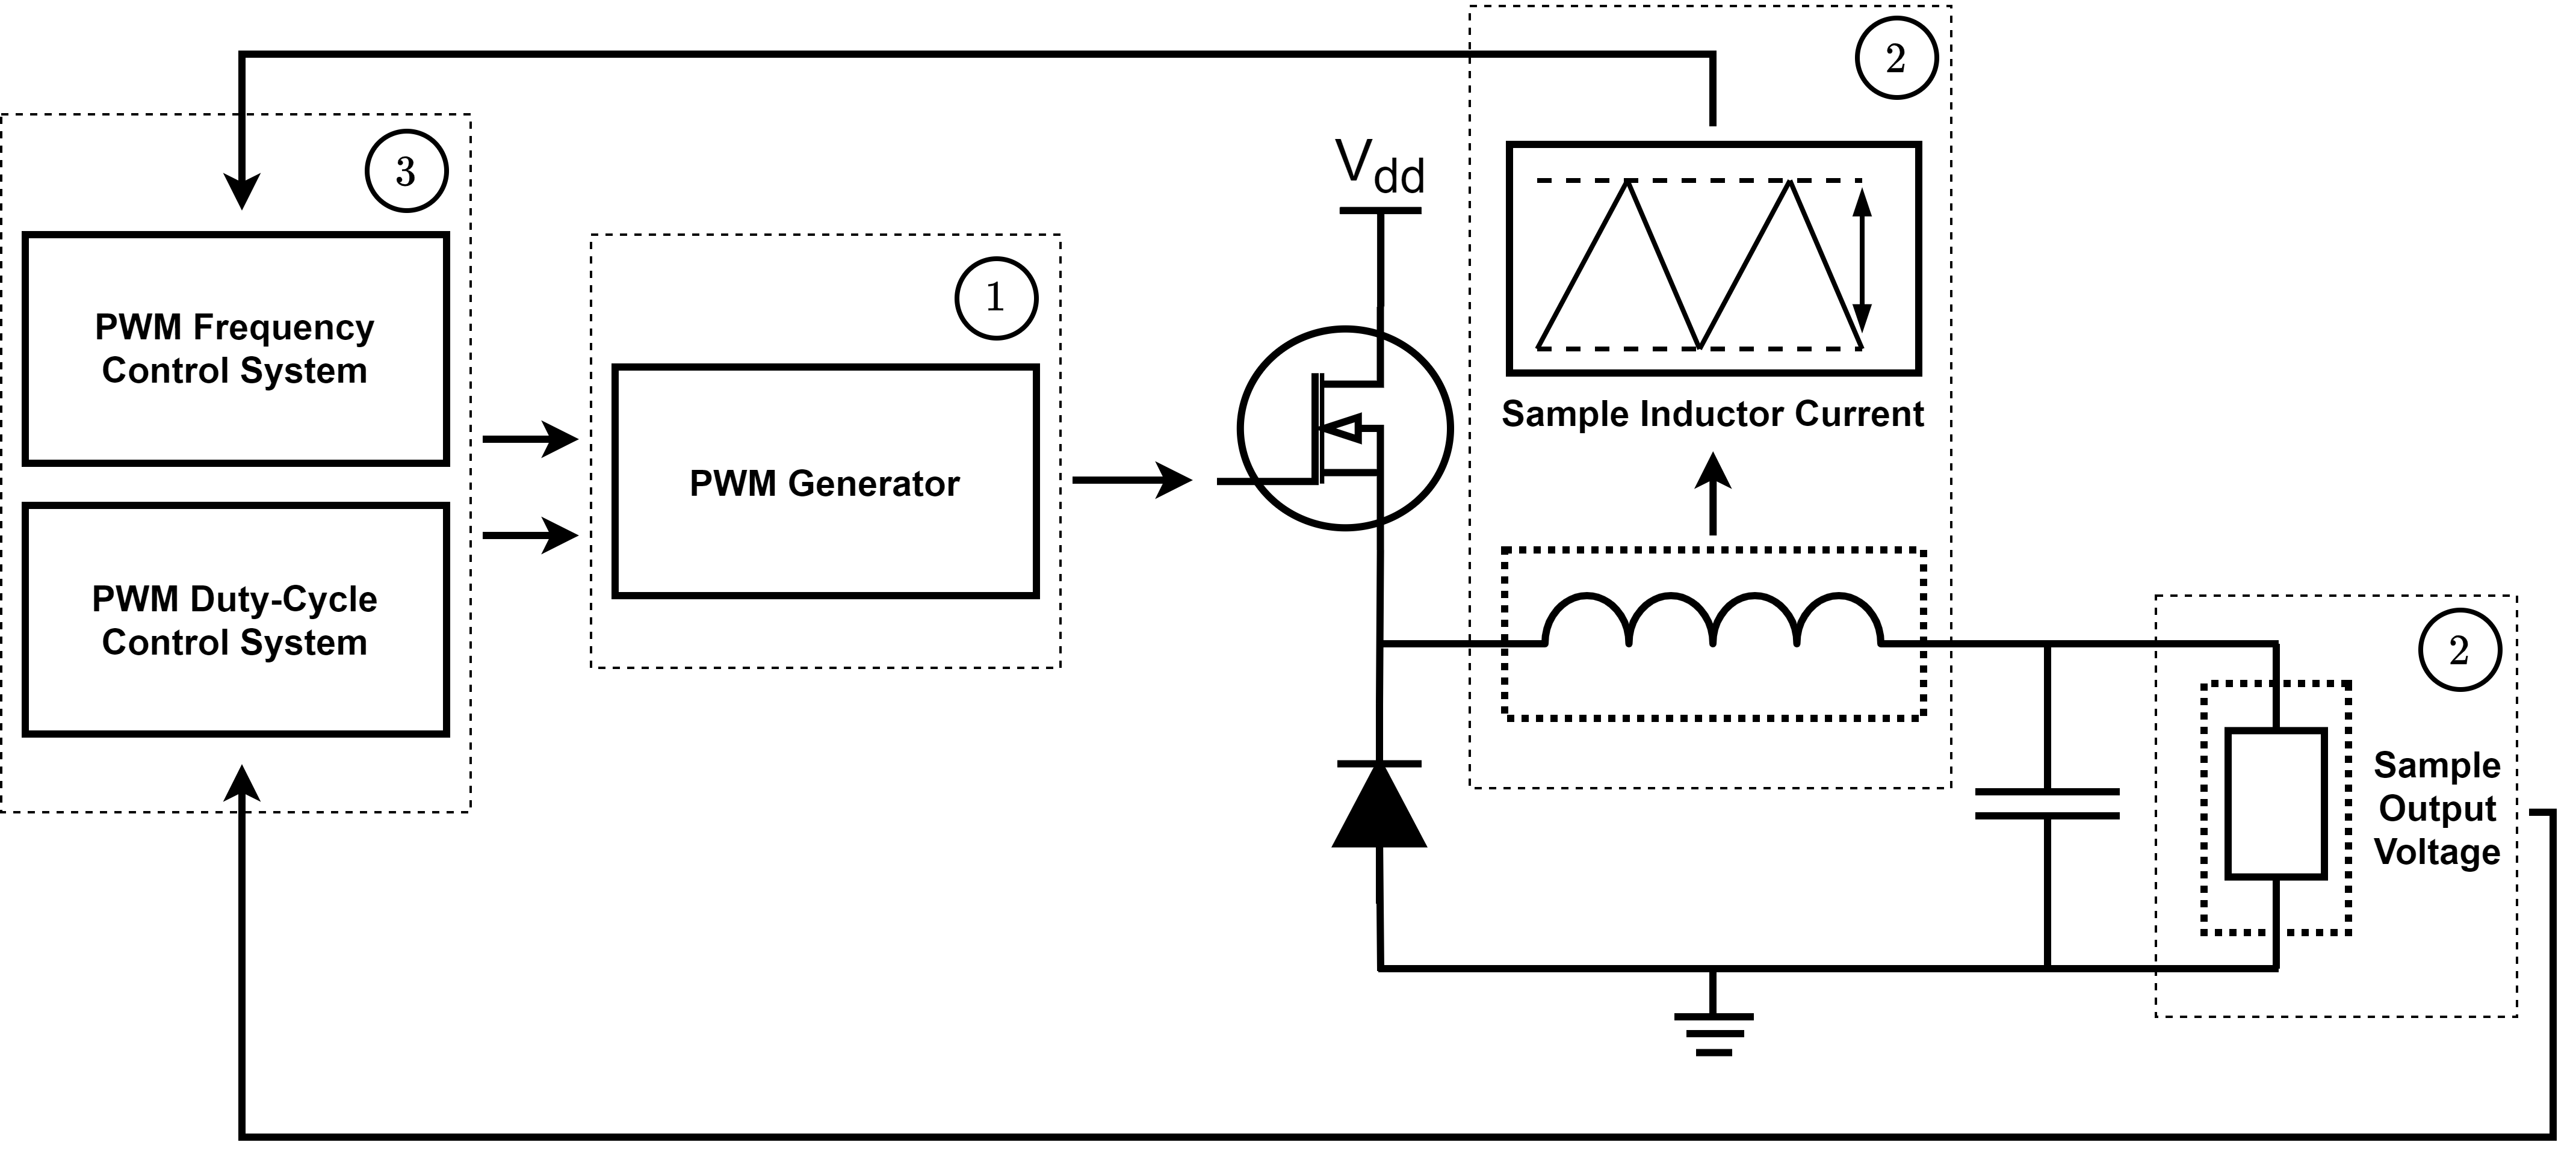
\includegraphics[width = 1\textwidth]{System_Overview.png}
    \caption{High level system overview}
    \label{F:sys_overview}
\end{figure}

\section{PWM Generation Design}\label{S:pwm_gen}

\begin{itemize}

    \item 
    Discuss the different PWM generation methods outlined in chapter \ref{C:background}. Talk about each of their specific design implication, their advantages, and their disadvantages. This will be included in three different sections, analogue, microcontroller, FPGA. 

    \item 
    Discuss why I have selected a microcontroller for the PWM generation. And discuss how the design of this implementation affected the microcontroller selection. 

    \item 
    Discuss how the final design of the PWM generation was implemented, and what it's capabilities are. Show some images of it functioning, and attach the esp32 code in the appendix.

\end{itemize}